\documentclass{article}
\usepackage{tikz}
\usetikzlibrary{arrows.meta}

\begin{document}

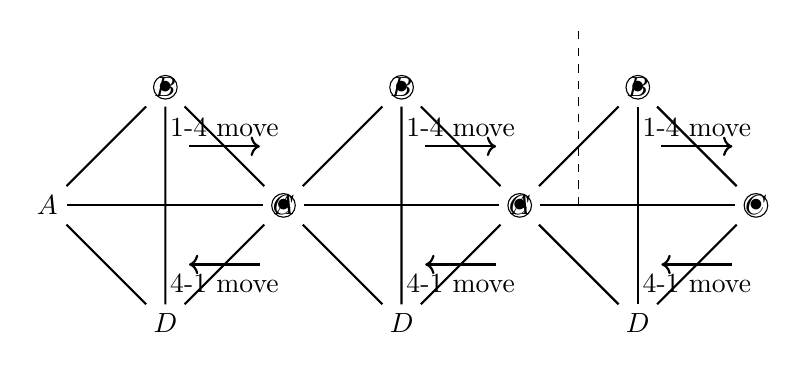
\begin{tikzpicture}[scale=1.5]
    % Define node positions
    \node (A) at (-2, 0) {$A$};
    \node (B) at (-1, 1) {$B$};
    \node (C) at (0, 0) {$C$};
    \node (D) at (-1, -1) {$D$};

    % Draw edges
    \draw[thick] (A) -- (B);
    \draw[thick] (A) -- (C);
    \draw[thick] (A) -- (D);
    \draw[thick] (B) -- (C);
    \draw[thick] (B) -- (D);
    \draw[thick] (C) -- (D);

    % Circle nodes
    \node[circle, draw, minimum size=0.3cm, inner sep=0pt, label=center:$\bullet$] at (B) {};
    \node[circle, draw, minimum size=0.3cm, inner sep=0pt, label=center:$\bullet$] at (C) {};

    % Arrows and labels
    \draw[->, thick] (-0.8, 0.5) -- (-0.2, 0.5) node[midway, above] {1-4 move};
    \draw[<-, thick] (-0.8, -0.5) -- (-0.2, -0.5) node[midway, below] {4-1 move};

    % Second diagram
    \begin{scope}[xshift=2cm]
        % Define node positions
        \node (A) at (-2, 0) {$A$};
        \node (B) at (-1, 1) {$B$};
        \node (C) at (0, 0) {$C$};
        \node (D) at (-1, -1) {$D$};

        % Draw edges
        \draw[thick] (A) -- (B);
        \draw[thick] (A) -- (C);
        \draw[thick] (A) -- (D);
        \draw[thick] (B) -- (C);
        \draw[thick] (B) -- (D);
        \draw[thick] (C) -- (D);

        % Circle nodes
        \node[circle, draw, minimum size=0.3cm, inner sep=0pt, label=center:$\bullet$] at (B) {};
        \node[circle, draw, minimum size=0.3cm, inner sep=0pt, label=center:$\bullet$] at (C) {};

        % Arrows and labels
        \draw[->, thick] (-0.8, 0.5) -- (-0.2, 0.5) node[midway, above] {1-4 move};
        \draw[<-, thick] (-0.8, -0.5) -- (-0.2, -0.5) node[midway, below] {4-1 move};
    \end{scope}

    % Third diagram
    \begin{scope}[xshift=4cm]
        % Define node positions
        \node (A) at (-2, 0) {$A$};
        \node (B) at (-1, 1) {$B$};
        \node (C) at (0, 0) {$C$};
        \node (D) at (-1, -1) {$D$};

        % Draw edges
        \draw[thick] (A) -- (B);
        \draw[thick] (A) -- (C);
        \draw[thick] (A) -- (D);
        \draw[thick] (B) -- (C);
        \draw[thick] (B) -- (D);
        \draw[thick] (C) -- (D);

        % Circle nodes
        \node[circle, draw, minimum size=0.3cm, inner sep=0pt, label=center:$\bullet$] at (B) {};
        \node[circle, draw, minimum size=0.3cm, inner sep=0pt, label=center:$\bullet$] at (C) {};

        % Arrows and labels
        \draw[->, thick] (-0.8, 0.5) -- (-0.2, 0.5) node[midway, above] {1-4 move};
        \draw[<-, thick] (-0.8, -0.5) -- (-0.2, -0.5) node[midway, below] {4-1 move};
    \end{scope}

    % Dashed line
    \draw[dashed] (2.5, 0) -- (2.5, 1.5);
\end{tikzpicture}

\end{document}